% Brian Mc George
% MCGBRI004
% 13/04/2015

\documentclass[]{article}
\title{Functional Programming Assignment 1\\Theoretical Questions}
\date{13-04-2015}
\author{Brian Mc George\\MCGRBRI004
}
\usepackage{graphicx}
\usepackage{amsfonts}
\usepackage{amsmath}
\usepackage{float}
\usepackage{tabularx}\begin{document}

\maketitle
\newpage

\section{How many non-distrinct states can be generated in \(n\) moves (Question 2.2)?}
The Rubik's cube can be twisted in six directions. For each state six new (non-distinct) states can be generated. \(n\) moves can be represented by the following mathematical function:
\begin{equation}\label{func_states}	
	f(n)=6^n\text{ for all }n \in\mathbb{N}
\end{equation}

\section{Investigate processing speed and memory usage for different values of \(n\) (Question 3.2)}
\subsection{Test System}
The tests were run on an Intel Core i7 2600 (3.4Ghz) processor running Windows 8.1 x64 using the gambit interpreter

\subsection{Effect of \(n\) On Completion Time}
\subsubsection{Testing Methodology}
Tests were conducted for \(n\) up to size 8.
The following function was used to test completion time and memory allocation\begin{equation*}\begin{split}
cubeSolve(rotationString) = \text{(time (solveCube solvedStates (rotate }rotationString \\\text{ '((1 1) (2 1) (3 1) (4 1) (5 3) (6 3) (7 3) (8 3))) 0))}
\end{split}\end{equation*}
The rotation string used for \(n = 8\) was "xyzXYZxy", for \(n = 7\) was "xyzXYZx" etc.\newline\newline The memory allocated would appear to be the memory allocated during the runtime not the total memory used at a particular time. It should be pointed out that this testing used the rotation optimisation outlined in Question 4. Secondly, to get faster completion time a non-tail recursive genStates method was used. Two implementations of genStates were written, one was tail recursive (completed slower) and the other was not tail recursive (completed faster). For comparison at a size \(n = 7\), solveCube with non-tail recursive genStates completed in 15 seconds with a peak memory usage of 740 MB. The solveCube with tail recursive genStates completed in 240 seconds with a peak memory usage of 273 MB. The non-tail recursive genStates was selected since the assignment brief outlined that it should be able to solve cubes of 7 moves or less. The memory usage only becomes a concern from at least 8 moves from which the tail recursive genStates would have to be used.
\subsubsection{Results Obtained}
\begin{table}[H]
\begin{center}
	\begin{tabular}{|r|c|l|}
		\hline
		Size of \(n\)&Memory Allocated (MB)&Completion Time (Seconds)\\
		\hline
		1&0.07728&\textless\space0.001\\
		2&0.556592&0.002\\
		3&3.48304&0.012\\
		4&21.130368&0.070\\
		5&128.346848&0.448\\
		6&786.701024&2.558\\
		7&4824.05504&15.853\\
		8&29659.645296&95.583\\
		\hline
		
	\end{tabular}\caption{Memory usage and completion time for different size of \(n\)}\end{center}
	\label{table:mem_usage}
\end{table}

 The results would indicate an exponential increase in running time and memory usage. The increase in running time could be as a result of the exponentially increasing search space to find the solution from. The increase in memory usage could be a result of it not being tail recursive as well as the search space, whose size is proportional to \(n\), that needs to be stored. 
 
 \subsection{Memory Usage During Runtime}
 \subsubsection{Testing Methodology}
 The \(cubeSolve\) function defined above was used with \(rotationString\) for \(n = 7\). Process Explorer was used to track the memory usage during program execution. This could be as a result of the genStates method not being tail recursive as the fact that the search space is expanding by a multiple of 5 as the depth increases.
 \subsubsection*{Results Obtained}
 
 % Memory Usage Image
 \begin{figure}[H]
 	\centering
 	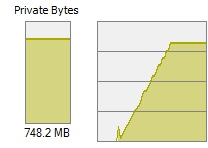
\includegraphics[width=0.4\linewidth]{mem_usage2.jpg}
 	\caption{Memory Usage Over Time (Non-Tail Recursive genStates)}
 	\label{fig:memory_usage}
 \end{figure}
  \begin{figure}[H]
  	\centering
  	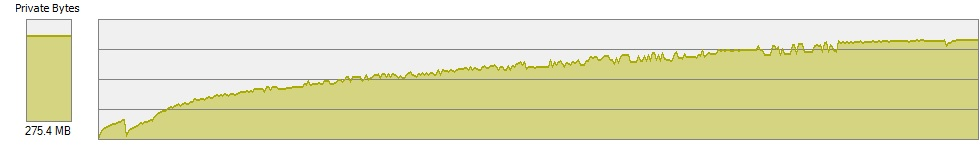
\includegraphics[width=1.2\linewidth]{mem_usage3.jpg}
  	\caption{Memory Usage Over Time (Tail Recursive genStates)}
  	\label{fig:memory_usageTail}
  \end{figure}
 Figure \ref{fig:memory_usage} shows a linear increase in memory usage as the program executes. Figure \ref{fig:memory_usageTail} shows a logarithmic increase in memory usage as the program executes. The tail recursive genStates is much more memory efficient that the tail recursive genStates. The length of the graph indicates that the solveCube using tail recursive genStates is much slower than than using the non-tail recursive genState. 

\section{Optimise algorithm and calculate reduction in number of states (Question 4)}
\subsection{Optimised function and number of states for \(n = 10\)}
Using function \ref{func_states}, the number of states that can be generated from 10 moves where 6 possible rotations can be made for each state is:
\begin{equation*}
\begin{split}
  f(10) & = 6^{10} \\
		  & = 60466176\text{ states}
\end{split}
\end{equation*}								
Function \ref{func_states} can be optimised such that from a given non-initial state, the new states generated are only those that will not undo the last move.
\begin{equation}
\begin{split}
g(n) =
\begin{cases}
	6^{n} & \text{if }n \in T = \{0, 1\}\\
	6 \times 5^{n-1} & \text{if }n \in \mathbb{N} \setminus T\\
	0 & \text{otherwise}
\end{cases}
\end{split}
\label{fun:func_states_optimised}
\end{equation}
Using function \ref{fun:func_states_optimised} the number of states generated from 10 moves is:
\begin{equation*}
\begin{split}
  g(10) & = 6 \times 5^{10-1} \\
		  & = 11718750\text{ states}
\end{split}
\end{equation*}
It follows that function \ref{fun:func_states_optimised} produces 48747426 (80.62\%) fewer states than function \ref{func_states}
\subsection{Results Of Optimisation}
\begin{table}[H]
	\begin{center}
		\noindent\makebox[\textwidth]{%
		\begin{tabular}{|r|c|c|c|c|}
			\hline
			Size of \(n\)&Memory Allocated (MB) &Memory Reduction (\%)&Completion Time (Seconds)& Completion Time Reduction (\%)\\
			\hline
			1&0.077504&-0.29&\textless\space0.001&0\\
			2&0.530832&4.63&0.002&0\\
			3&2.895664&16.86&0.09&25.00\\
			4&14.866848&29.64&0.046&34.29\\
			5&75.620656&41.08&0.251&43.97\\
			6&382.531696&51.38&1.299&49.22\\
			7&1945.344192&59.67&6.336&60.03\\
			8&10000.118816&66.28&31.641&66.90\\
			\hline
			
		\end{tabular}}\caption{Memory usage and completion time for different size of \(n\)}\end{center}
	\label{table:mem_usage}
\end{table}
\end{document}
